\documentclass{article}
\usepackage[utf8]{inputenc}

\usepackage{amsthm,amssymb,amsmath}
\usepackage{graphicx}
\usepackage{float}
\usepackage{caption, subcaption}
\usepackage{hyperref}

\newcommand{\NN}{\mathbb{N}}
\newcommand{\ZZ}{\mathbb{Z}}
\newcommand{\RR}{\mathbb{R}}
\newcommand{\QQ}{\mathbb{Q}}
\newcommand{\CC}{\mathbb{C}}

\title{AERO7970 - Trajectory Optimiztion \\ {\small Project 04}}
\author{Matt Boler}
\date{\today}

\begin{document}

\maketitle

\begin{abstract}
  This report details the implementation of an obstacle-avoiding trajectory solver using successive convexification.
  The solver was implemented in \texttt{Matlab} using both the built-in \texttt{coneprog} solver and the open-source \texttt{CVX} solver.
  The trajectories, commanded control inputs, and runtimes of the two solvers are compared.
\end{abstract}

\section{Introduction}

We are given the task of applying \textit{successive convexification} (SCvx)\cite{mao_successive_2019} to generate optimal trajectories between two points while avoiding obstacles.
SCvx is a method of solving non-convex problems by iteratively approximating the original problem as a locally convex problem.
In this case, requiring the trajectory to avoid obstacles makes the search space non-convex.
An example of the problem is shown below in Figure \ref{fig:example}.

\begin{figure}[H]
  \centering
  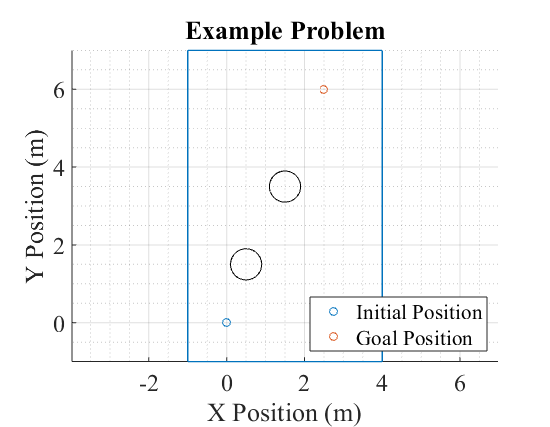
\includegraphics[width=0.7\textwidth]{images/example.png}
  \caption{An example obstacle avoidance problem}
  \label{fig:example}
\end{figure}

%%
\section{Problem Modeling}

The optimization problem is given by Problem 2 of Szmuk et. al \cite{szmuk_convexification_2017}.
The platform dynamics are modeled as a 3DOF $2^{nd}$-order integrator and the commanded thrust is bounded above and below.
Initial and final conditions are given.
The optimization problem is reproduced below in Equation \ref{eq:problem}.

\begin{align} \label{eq:problem}
  \min_{u^k(t), \Gamma^k(t)} \quad & w \int_t^{t_f} (\Gamma^k(t)^2)dt + \sum_{j \in \mathbb{J}} \nu_j \\
  \textrm{s.t.} \quad & r^k(0) = r_i, \quad v^k(0) = 0, \quad u^k(0) = g e_3 \nonumber \\
  & r^k(t_f) = r_f, \quad v^k(t_f) = 0, \quad u^k(t_f) = g e_3 \nonumber \\
  & \dot{r}^k(t) = v^k(t) \nonumber \\
  & \dot{v}^k(t) = u^k(t) \nonumber \\
  & ||u^k(t)||_2 \leq \Gamma^k(t) \nonumber \\
  & 0 < u_{min} \leq \Gamma^k(t) \leq u_{max} \nonumber \\
  & \Gamma^k(t) \cos(\theta_{max}) \leq e_3^T u^k(t) \nonumber \\
  \forall j \in \mathbb{J}, \quad t \in [0, t_f]:& \nonumber \\
  & \nu_j \geq 0 \nonumber \\
  & H_j \succeq 0 \nonumber \\
  & \Delta r^{k, j}(t) \triangleq ( r^{k-1}(t) - p_j ) \nonumber \\
  & \delta r^k(t) \triangleq ( r^k(t) - r^{k-1}(t) ) \nonumber \\
  & \xi^{k,j} \triangleq ||H_j \Delta r^{k,j}(t)||_2 \nonumber \\
  & \zeta^{k,j} \triangleq \frac{H_j^T H_j \Delta r^{k,j}(t)}{\xi^{k,j}} \nonumber \\
  & \xi^{k,j} + \zeta^{k,j}(t)^T \delta r^k(t) \geq R_j - \nu_j \label{eq:linearized_constraints}
\end{align}
where Equation \ref{eq:linearized_constraints} and the preceding lines describe the relaxed obstacle constraints for each obstacle $p_j \in \mathbb{J}$.

In order to solve using SCvx, an initial solution is required.
We find this initial solution by solving Equation \ref{eq:problem} without the linearized obstacle constraints to find $\hat{r}$, $\hat{v}$, $\hat{u}$, and $\hat{\Gamma}$.
These solutions are then used as the previous solution for the first iteration of SCvx.

\section{Results}

\subsection{Coneprog Solver}

SCvx was first implemented in \texttt{Matlab} using the built-in \texttt{coneprog} solver and a problem-based approach.
Of note, while minimization of a squared norm can be converted from a quadratic problem to a second-order cone program, \texttt{coneprog} will not do this for you.
To do so, a slack variable $Y$ was introduced to bound the quadratic term as described in \href{https://www.mathworks.com/help/optim/ug/convert-qp-to-socp.html}{Mathworks documentation}.
Generated trajectories and control efforts from \texttt{coneprog} are shown below in Figures \ref{fig:coneprog_trajectories} and \ref{fig:coneprog_controls}.

\begin{figure}[H]
  \centering
  \begin{subfigure}{.5\textwidth}
    \centering
    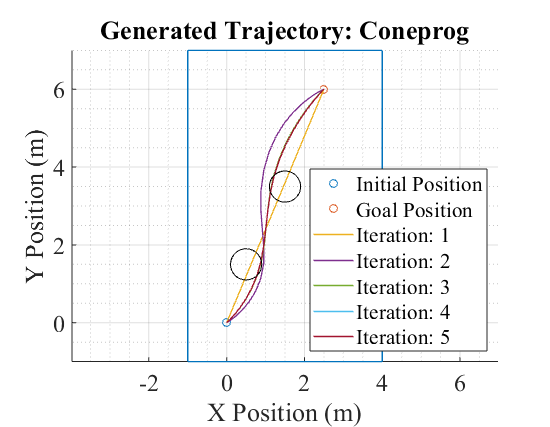
\includegraphics[width=\linewidth]{images/coneprog/traj1_trajectories.png}
    \label{fig:coneprog_traj1}
  \end{subfigure}%
  \begin{subfigure}{.5\textwidth}
    \centering
    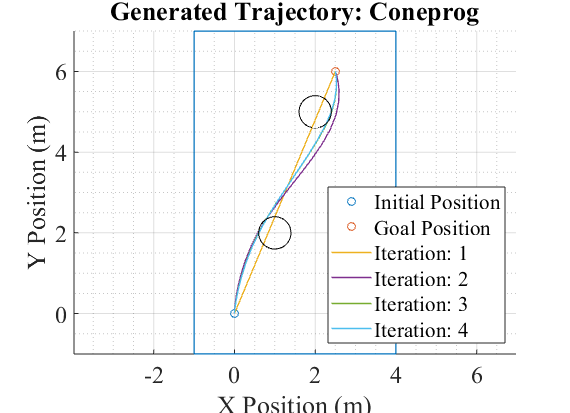
\includegraphics[width=\linewidth]{images/coneprog/traj2_trajectories.png}
    \label{fig:coneprog_traj2}
  \end{subfigure}
  \caption{Trajectories generated with \texttt{coneprog}}
  \label{fig:coneprog_trajectories}
\end{figure}

\begin{figure}[H]
  \centering
  \begin{subfigure}{.5\textwidth}
    \centering
    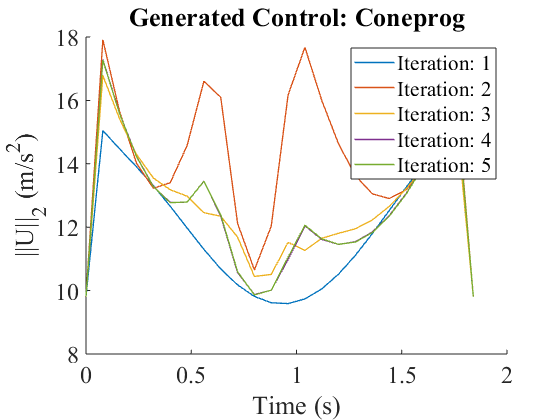
\includegraphics[width=\linewidth]{images/coneprog/traj1_control.png}
    \label{fig:coneprog_contr1}
  \end{subfigure}%
  \begin{subfigure}{.5\textwidth}
    \centering
    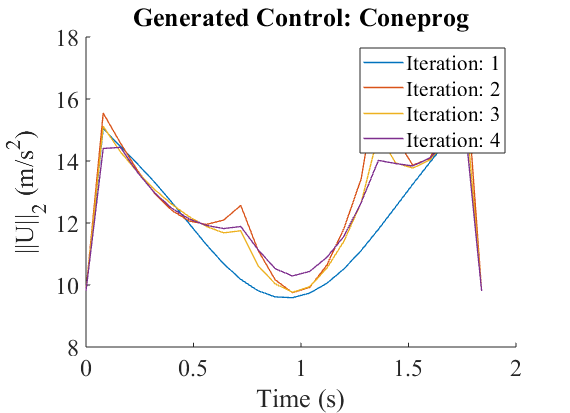
\includegraphics[width=\linewidth]{images/coneprog/traj2_control.png}
    \label{fig:coneprog_contr2}
  \end{subfigure}
  \caption{Control commands generated with \texttt{coneprog}}
  \label{fig:coneprog_controls}
\end{figure}

\subsection{CVX Solver}

Next, SCvx was implemented in the open-source convex optimization toolbox \texttt{CVX}.
\texttt{CVX} has several built-in niceties such as automatic conversion of quadratic programs with SOCP constraints to SOCP programs.
As a result, SCvx was able to be implemented as in Equations \ref{eq:problem} and \ref{eq:linearized_constraints} without modification.
Generated trajectories and control efforst from \texttt{CVX} are shown below in Figures \ref{fig:cvx_trajectories} and \ref{fig:cvx_controls}.

\begin{figure}[H]
  \centering
  \begin{subfigure}{.5\textwidth}
    \centering
    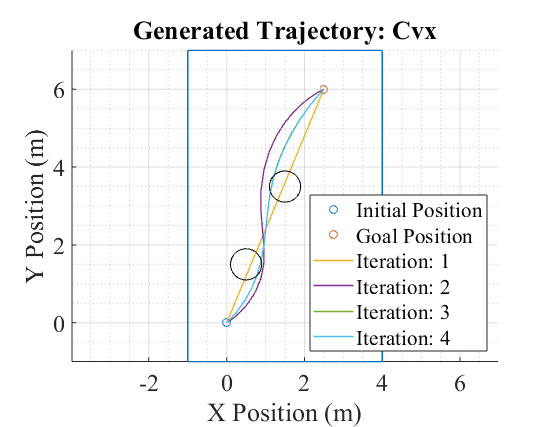
\includegraphics[width=\linewidth]{images/cvx/traj1_trajectories.png}
    \caption{A subfigure}
    \label{fig:cvx_traj1}
  \end{subfigure}%
  \begin{subfigure}{.5\textwidth}
    \centering
    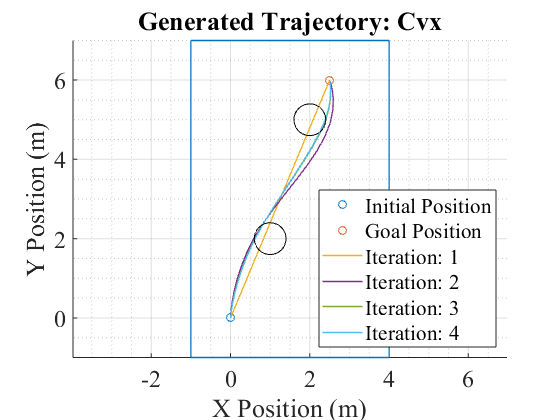
\includegraphics[width=\linewidth]{images/cvx/traj2_trajectories.png}
    \caption{A subfigure}
    \label{fig:cvx_traj2}
  \end{subfigure}
  \caption{Trajectories generated with \texttt{CVX}}
  \label{fig:cvx_trajectories}
\end{figure}

\begin{figure}[H]
  \centering
  \begin{subfigure}{.5\textwidth}
    \centering
    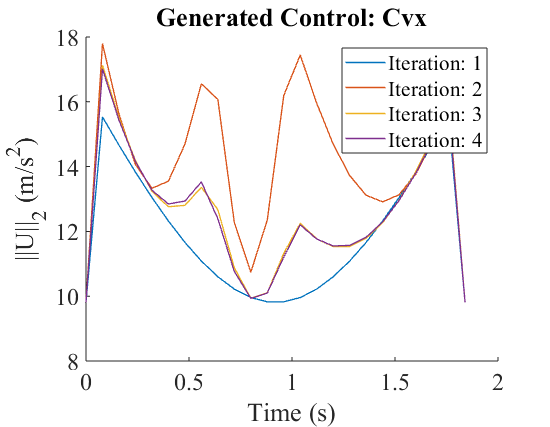
\includegraphics[width=\linewidth]{images/cvx/traj1_controls.png}
    \label{fig:cvx_contr1}
  \end{subfigure}%
  \begin{subfigure}{.5\textwidth}
    \centering
    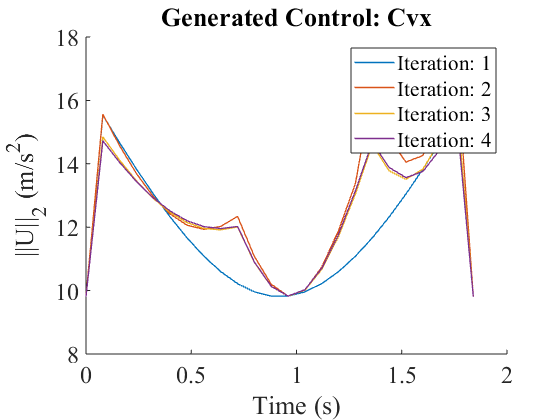
\includegraphics[width=\linewidth]{images/cvx/traj2_controls.png}
    \label{fig:cvx_contr2}
  \end{subfigure}
  \caption{Control commands generated with \texttt{CVX}}
  \label{fig:cvx_controls}
\end{figure}

\subsection{Performance Comparison}

The performance results of the two implementations are shown below.
The \texttt{coneprog} solver is about 1 second faster than the \texttt{CVX} solver on average.

\begin{figure}[H]
  \begin{verbatim}
Testing ConeProg performance
  - Iteration: 1, 1.6008
  - Iteration: 2, 1.5742
  - Iteration: 3, 1.569
  - Iteration: 4, 1.5223
  - Iteration: 5, 1.5066
  - Iteration: 6, 1.5125
  - Iteration: 7, 1.5437
  - Iteration: 8, 1.5087
  - Iteration: 9, 1.4817
  - Iteration: 10, 1.4791
Average time to solve with ConeProg: 
    1.5299
  \end{verbatim}
  \caption*{Performance results from \texttt{coneprog} implementation of SCvx}
\end{figure}

\begin{figure}[H]
  \begin{verbatim}
Testing CVX performance
  - Iteration: 1, 2.3492
  - Iteration: 2, 2.3063
  - Iteration: 3, 2.3183
  - Iteration: 4, 2.2605
  - Iteration: 5, 2.2148
  - Iteration: 6, 2.1939
  - Iteration: 7, 2.2043
  - Iteration: 8, 2.2814
  - Iteration: 9, 2.3704
  - Iteration: 10, 2.1954
Average time to solve with CVX: 
    2.2695
  \end{verbatim}
  \caption*{Performance results from \texttt{CVX} implementation of SCvx}
\end{figure}

\section*{Conclusion}

This report has presented results from implementing SCvx using two SOCP solvers.
While the \texttt{coneprog} implementation runs faster than the \texttt{CVX} implmentation, the \texttt{CVX} implementation was significantly easier to write, test, and generally work with.
I spent around 25 hours on this project.

\bibliographystyle{plain}
\bibliography{project4}

\end{document}
